% https://mipt.ru/education/departments/lpr/students/theses.php

% document's head

\begin{center}
    \LARGE \textsc{Желательные знания по курсу <<Физическая кинетика>>}
\end{center}

\hrule

\phantom{42}

\begin{flushright}
    \begin{tabular}{rr}
    % written by:
        % \textbf{Источник}: 
        % & \href{__ссылка__}{__название__} \\
        % & \\
        % \textbf{Лектор}: 
        % & _ФИО_ \\
        % & \\
        \textbf{Автор заметок}: 
        & Хоружий Кирилл \\
        & \\
    % date:
        \textbf{От}: &
        \textit{\today}\\
    \end{tabular}
\end{flushright}

\thispagestyle{empty}
\tableofcontents
\newpage


\newpage
\subsection*{\xmark Аннотация}
\addcontentsline{toc}{section}{Аннотация}
% -- аннотация (отражаются цели и задачи работы и полученные результаты, в
% дальнейшем размещается в открытом доступе, не более 1500 знаков);


В работе исследованы методы охлаждения атомов и их загрузки в магнито-оптическую ловушку (МОЛ) с помощью зеемановского замедлителя (ЗЗ) и оптической патоки (ОП). Была построена модель охлаждения атомов с помощью ЗЗ и их дальнейшей загрузки в систему ОП+МОЛ. На основе построенной модели оптимизированы параметры магнитного поля и лазерного излучения ЗЗ, ОП, МОЛ, что привело к повышению эффективности охлаждения и позволило уменьшить температуру печи и увеличить время непрерывной работы установки в 5 раз. Также была рассмотрена альтернатива ЗЗ - двухмерная магнито-оптическая ловушка (2D-МОЛ), которая представляет более компактную альтернативу ЗЗ при сохранении потока загрузки МОЛ. 


% \newpage
% \tableofcontents


\unewpage
\section*{Обозначения и сокращения}
\addcontentsline{toc}{section}{Обозначения и сокращения}


 
\begin{tabular}{lll}
	МОЛ & магнито-оптическая ловушка & \pageref{subsec:мол} \\ 
	2D-МОЛ  & двухмернная магнито-оптическая ловушка & \\ 
	ЗЗ & зеемановский замедлитель & \\
	АОМ & акусто-оптический модулятор & \\
	СВВ & сверхвысокий вакуум & \\
	$\alpha$ & наиболее вероятная тепловая скорость атомов & \pageref{Поток атомов на выходе}\\ 
	$\sub{v}{slow}$ &  характерная скорость замедленных в ЗЗ атомов & \pageref{Тормозящая сила} \\
	$\sub{v}{crit}$ & максимальная скорость атомов, при которой ЗЗ эффективно работает  & \pageref{Тормозящая сила} \\
	$\sub{v}{cap}$ & скорость захвата МОЛ & \pageref{Эффективность замедлителя}, \pageref{Поток загрузки} \\
	$\sub{\Phi}{tot}$ & поток атомов, вылетающих из печки & \\
	$\sub{\Phi}{sol}$ & поток атомов, влетающих в ЗЗ & \pageref{Поток атомов на выходе} \\
	$\sub{\Phi}{load}$ & поток загрузки МОЛ & \pageref{Динамика количества атомов в МОЛ} \\
\end{tabular}





%%%%%%%%%%%%%%%%%%%%%%%%%%%%%%%%%%%%%%%%%%%%%%%%%%%%%%%%%%%%%%%%%%%%%%%%%%%%%%%%
\unewpage
\section{Введение}



\begin{minipage}{0.25\textwidth}
Квантовые приборы:
\begin{itemize}
	\iitem{гравиметры}
	\iitem{часы}
	\iitem{транспортиры}
	\iitem{...}
	\iitem{...}
\end{itemize}
\end{minipage}
\hfill
\begin{minipage}{0.7\textwidth}
\textbf{Квантовые симуляторы}:
\begin{itemize}
	\iitem{реализация моделей ферми-хаббарда и бозе-хаббарда}
	\iitem{переход от БКШ к БЭК}
	\iitem{локализация Андерсона и многочастичная локализация}
	\iitem{формирование вихрей в БЭК}
	\iitem{...}
\end{itemize}
\end{minipage}


\phantom{42}

\phantom{42}




%%%%%%%%%%%%%%%%%%%%%%%%%%%%%%%%%%%%%%%%%%%%%%%%%%%%%%%%%%%%%%%%%%%%%%%%%%%%%%%%
\subsection{Области применения ультрахолодных атомов}
В области ультрахолодных атомов можно выделить две принципиальные области применений: создание сверхточных измерительных приборов и квантовая симуляция многочастичных систем. Создание квантовых симуляторов позволяет исследовать процессы, недоступные к аналитическому описанию или численному моделированию, в связи с экспоненциальным ростом сложности вычислений многочастичных задач в квантовой механике. Высокая точность измерений связана с возможностью работать с системами в их основном состоянии и наблюдению интерференционных явлений.и





% про измерения
Физика ультрахолодных атомов позволяет добиваться сверхточного измерения времени. Стандарт секунды определяется переходом в атоме ${}^{133}$Cs, реализация часов на основе лазерного охлаждения позволяет достигать точности порядка $10^{-16}$ \cite{schmittberger2020review, 799241}. На Sr и Yb получены точности порядка $10^{-18}$ \cite{schmittberger2020review, Bloom_2014}. 

Измерение гравитационных эффектов с помощью ультрахолодных атомов находит применение в фундаментальных исследованиях \cite{Tino_2021} измерение гравитационной постоянной $G$, исследование гравитации на малых масштабах, измерение параметра Этвёша; развиваются детекторы гравитационных волн на основе атомных интерферометров \cite{Dimopoulos_2009}. Измерение ускорения свободного падения может использоваться для практических задач, например поиска месторождений полезных ископаемых \cite{Tino_2021}.




% про симуляторы в общем
Основой квантовых симуляторов на ультрахолодных атомах является возможность в широком диапазоне настраивать различные параметры системы, такие как сила взаимодействия атомов \cite{bloch2012quantum}
, структура и глубина потенциала решетки \cite{lewenstein_ultracold_2007, gross_quantum_2017, tsyganok2023boseeinstein}, в которую помещаются охлажденные атомы, температуру и концентрацию. В зависимости от используемых атомв возможна симуляция ферми или бозе систем, а также их смесей \cite{yamamoto2012lattice}. С использованием объективов с большой числовой апертурой возможно получение разрешения в один узел оптической решётки \cite{Sherson_2010}, что позволяет напрямую наблюдать исследуемые явления на микроскопическом масштабе, увеличивая точность экспериментов и качественно меняя доступные к измерениям эффекты.  

В исследуемых с помощью квантовых симуляторов особенно можно выделить многочастичные задачи в оптических решётках \cite{bloch_many-body_2008}, формально реализующие модель ферми-хаббарда и бозе-хаббарда (с реализацией, например, перехода от сверхтекучести к моттовскому изолятору \cite{Greiner2002}). Экспериментально наблюдались вихри во вращающемся бозе-конденсате, формирование вихрями решётки \cite{Klaus_2022}.  Возможность настройки взаимодействия через резонанс Фешбаха позволяет исследовать переход от сверхтекучести БКШ, когда притяжение слабое и спаривание проявляется только в импульсном пространстве, к конденсату Бозе-Эйнштейна тесно связанных пар в реальном пространстве \cite{bloch_many-body_2008}.

Особый интерес представляет исследование условий, когда система не термализуется \cite{abanin_colloquium_2019}, так как это является важным шагом на пути к пониманию новых состояний материи, которые могут возникать в сильно неравновесных квантовых системах. Основным путём к термолизации является рассеивание энергии по доступным степеням свободы, что требует переноса между разными частями системы. Соответсвенно нарушение эргодичности происход в изолирующих системах. Примерами такого изолюирующего поведения, исследуемого с помощью квантовых симуляторов на ультрахолодных атомах, являются андерсоновская локализация \cite{roati_anderson_2008} и многочастичная локализация \cite{choi_exploring_2016}.


\unewpage
\subsection{\xmark Актуальность проблемы}
При реализации квантового симулятора на атомах Tm в нашей лаборатории возникла следующая проблема: из-за большого потока атомов из печи, на зеркало, которое находится напротив печи, напыляются атомы. Этот процесс приводит к ухудшению отражательных свойств зеркала, уменьшению стабильности установки и существенному ограничению времени жизни установки. В данной работе описано решение этой проблемы, путём уменьшения потока атомов из печи, при сохранение потока загрузки МОЛ. Оптимизация количества атомов Tm в МОЛ позволила сохранить поток атомов, загружающихся в МОЛ. Также в работе рассматривается альтернативное решение проблемы напыления атомов тулия: использование источника охлажденного атомарного пучка Tm, не требующего встречного лазерного пучка. Основой альтернативного источника является 2D-МОЛ.

\unewpage
\subsection{Цели и задачи работы}
% ПОСТАНОВКА ЗАДАЧИ
% Здесь надо максимально формально описать суть задачи, которую потребуется решить, так, чтобы можно было потом понять, в какой степени полученное в результате работы решение ей соответствует. Текст главы должен быть написан в стиле
% технического задания, т.е. содержать как описание задачи, так и некоторый набор
% требований к решению


% \startp
% \upar{Печь}
% На данный момент хочется провести калибровку по температуре для печи. Для этого смотрим на мощность флюоресценции на выходе из печи, как на функцию температуры. Сравниваем с исходной калибровкой и калибровкой, полученной по точкам плавления меди и алюминия. 

% \upar{Зееман}
% Варьируя параметры отстройки и мощности, добиться такой же загрузки МОЛ при сохранение количества атомов в МОЛ. Найти, как от параметров зеемана зависит $\sub{v}{crit}$, $\sub{v}{cool}$, $\sub{\dot{N}}{cool}$.


Целями данной работы являлись оптимизация количества атомов ${}^{169}$Tm в магнитооптической ловушке, работающей на длине волны 530.7 нм: увеличение длительности работы источника атомов (печи), повышение эффективности процесса замедления атомов, а также проектирование альтернативного источника охлажденного атомарного пучка на двухмерной магнитооптической ловушке и оценка эффективности альтернативного источника.

В рамках работы были поставлены и решены следующие задачи 
\begin{enumerate*}
	\item С помощью спектроскопии атомарного пучка откалибровать температуру используемой в установке печи. Оптимизировать температуру печи.
	\item Построить модель замедления атомов в ЗЗ. Определить оптимальные параметры мощности лазерного луча, отстройки луча ЗЗ и значения токов в катушках ЗЗ. 
	\item Определить оптимальную отстройку для пучков МОЛ. Измерить значение потока загрузки МОЛ с помощью ЗЗ. 
	\item Построить модель формирования атомарного пучка в двухмерной магнитооптической ловушке. Определить оптимальные параметры мощности, отстройки, размеров пучка патоки. Расчитать ожидаемое значение потока загрузки МОЛ с помощью 2D-МОЛ. Рассмотреть возможное улучшение 2D-МОЛ до конфигурации 2D${}^+$МОЛ, когда используются лазерные пучки различной мощности. 
\end{enumerate*}




\subsection{Обзор существующих решений}
\vspace{2cm}



% Обзор существующих решений
% Здесь надо рассмотреть все существующие решения поставленной задачи, но не просто пересказать, в чем там дело, а оценить степень их соответствия тем ограничениям, которые были сформулированы в постановке задачи.

% монте-карло для зеемана
% 2d-мол
% 

\subsection{Роль автора}
Все результаты, изложенные в работе, получены лично автором либо при его решающем участии.
\subsection{Структура последующих глав}
\vspace{2cm}



% Обзор существующих решений
% Здесь надо рассмотреть все существующие решения поставленной задачи, но не просто пересказать, в чем там дело, а оценить степень их соответствия тем ограничениям, которые были сформулированы в постановке задачи.

% монте-карло для зеемана
% 2d-мол
% 







%%%%%%%%%%%%%%%%%%%%%%%%%%%%%%%%%%%%%%%%%%%%%%%%%%%%%%%%%%%%%%%%%%%%%%%%%%%%%%%%
\unewpage
\section{Экспериментальная установка}
%%%%%%%%%%%%%%%%%%%%%%%%%%%%%%%%%%%%%%%%%%%%%%%%%%%%%%%%%%%%%%%%%%%%%%%%%%%%%%%%
% опринципиальная схема установки
% общее описание работы приборчиков

Получение ультрахолодного облака атомов Tm происходит в несколько этапов, принципиальная схема приведена на рис.  \ref{fig:expT}.

\begin{figure}[h]
    \centering
    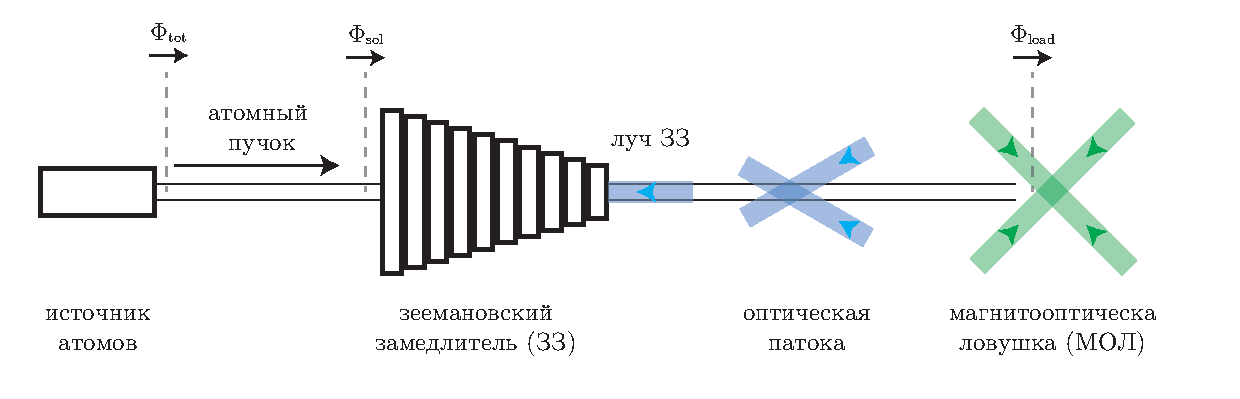
\includegraphics[width=1.0\textwidth]{figs/sheme.pdf}
    \caption{Принципиальная схема установки}
    \label{fig:expT}
\end{figure}


\begin{enumerate}
    \item Источник атомов (печь). Внутри высокого вакуума (ВВ) расположен тигель в печи с кусочком Tm, температура контролируется термопарой. В установке не достигается температура плавления Tm (1545 $\dC$), так что кусочек остаётся в твёрдом состоянии, с его поверхности происходит сублимация атомов, фомируя газ атомов Tm с давлением порядка давления насыщенных паров. Поток атомов из печи далее упоминается как $\sub{\Phi}{tot}$.
    \item Атомы вылетают из сопла печи, и попадают в зеемановский замедлитель (ЗЗ). Для охлаждения атомов используется встречный резонансный лазерный пучок на длине волны 410.6 нм (переход $\ket{F=4} \to \ket{F=5}$) и мощности порядка 70 мВт, магнитнымии катушками создаётся градиент магнитого поля (рис. \ref{fig:zB}) так, чтобы вдоль всей длины ЗЗ атомы выходящие из резонанса из-за доплеровского сдвига, оставались бы в резонансе за счёт зеемановского сдвига.  Поглощая фотоны атомы замедляются, т.к. дальнейшее переизлучение происходит изотропно. 
    \item После прохождения ЗЗ атомы дополнительно тормозятся встречными лучами оптической патоки, для охлаждения используется порядка 15 мВт излучения на длине волны 410.6 нм. С помощью АОМ добивается отстройка от атомного резонанса порядка $\Gamma$ \red{(уточнить)}. Механизм замедления аналогичен ЗЗ, однако наличие дополнительных охлаждающих встречных пучков перед МОЛ позволяет существенно увеличить скорость захвата системы оптическая патока + МОЛ. 
    \item После оптической патоки происходит захват в МОЛ, на длине волны 530.7 нм, общая потребляемая мощность лазерного излучения порядка 370 мВт, отстройка от резонанса порядка $10\Gamma$. Резонансным лазерным излучением создаётся замедляющая сила, аналогичная вязкому трению, вместе с используемыми в антигельмгольцевской конфигурации катушками, в нуле магнитного поля создаётся минимум потенциала. 
\end{enumerate}


\unewpage
\subsection{Калибровка температуры печи}

\startp
\upar{Определение температуры по потоку атомов}
Для определения температуры печи используется термопара, позволяющаю находить относительное изменение температуры, однако абсолютное значение $T_0$ было не откалибровано. Для калибровки термопары использовался следующий метод. Атомарный пучок, выходящий из печи, подсвечивался резонансным лазерным излучением на длине волны $410.6$ нм, соответсвтвующей переходу 410.6 нм \cite{vlad}. Фотодиодом измерялось значение флюоресценции  $\subt{V}{PD}$ атомов в пучке для различных значений отстройки лазера $\delta$ (рис. \ref{fig:oven}а). В резонансе максимум интенсивности пропорционален потоку атомов $\sub{\Phi}{tot}  \propto \sub{n}{sat}(T) $. Зависимость  $\sub{n}{sat}(T)$ приведена в \eqref{nTp}.

% Из зависимости \eqref{oven} видно, что $\sub{\Phi}{tot}(T)$ и, соответственно, экспоненциально зависит от температуры .


\begin{figure}[ht]
    \centering
    \subfigure[]{\includegraphics{figs/ovenD_v2.pdf}}
    \hspace{5 mm} 
    \subfigure[]{\includegraphics{figs/oven1_v4.pdf}}
    % \subfigure[]{\includegraphics{figs/oven2_v4.pdf}}
    \subfigure[]{\includegraphics[width=0.25\textwidth]{figs/photo.jpg}}
    \vspace{-3mm}
    \caption{a) Снятая экспериментальная зависимость мощности флюоресценции атомарного пучка от величины отстройки от резонанса лазерного излучения. Непрерывным линиями показана аппроксимация данных лоренцовым контуром. б) Относительная зависимость потока атомов из печки $\sub{\Phi}{tot}$ от температуры: черными точками отмечены экспериментально снаятые точки, непрерывными линиями отмечены границы линейной апроксимации  в) Фотография напыленного на стекло алюминия при достижении температуры плавления}
    \label{fig:oven}
\end{figure}


Найдём логарифмическую производную $\sub{\Phi}{tot}'/\sub{\Phi}{tot}$, с помощью линейной аппроксимации зависимости $\ln \sub{\Phi}{tot} (T)/ \sub{\Phi}{0}$ (рис. \ref{fig:oven}б), где $\Phi_0 = \sub{\Phi}{tot}(T=T_0 - 20 \dC)$. Решая уравнение $\sub{n}{sat}'/\sub{n}{sat} = \sub{\Phi}{tot}'/\sub{\Phi}{tot} = \subt{V}{PD}' / \subt{V}{PD}$, находим  $T_0 = (590 \pm 10) \dC$.
% \red{(полученное значение согласуется с экспериментом по реперной точке на температуре плавления алюминия, стоит ли эту историю описывать?)}.

\upar{Определение температуры по реперной точке} 
Абсолютное значение температуры было проверено и другим способом. В тигель печи помещался кусочек алюминия, затем постепенно увеличивалась температура. При достижении температуры $T_0 + 65 \dC$ на окошко перед печью напылялся Al, что соответсвует температуре плавления $660 \dC$ и значению $T_0 = 595 \dC$, в соглавсовании с первым методом.




\unewpage
\subsection{Обработка фотографии}
Для получения информации об атомном облаке в МОЛ использовалась схема изображенная на рис. \ref{fig:exp_photo}. 

\begin{figure}[h]
    \centering
    \includegraphics[width=0.9\textwidth]{figs/detect.png}
    \caption{Схема детектирования из \cite{vlad}}
    \label{fig:exp_photo}
\end{figure}


В соответствии с законом Бугера-Ламберта-Бера интенсивность резонансного лазерного пучка после прохождения через облако может быть найдена в виде
\begin{equation}
    \frac{d I}{d z} = - \sigma n I,
    \hspace{10 mm} 
    \sigma = \frac{\sigma_0}{1+I/I_s + 4 (\delta/\Gamma)^2},
\end{equation}
где $I_s$ -- интенсивность насыщения, $\delta$ -- отстройка от резонанса, $n$ -- концентрация атомов в ловушке, $\sigma_0 = 3 \lambda^2 / 2\pi$ -- резонансное сечение поглощения атомом одиночного фотона, $\lambda$ -- длина волны света. Для измерения параметров атомного облага с помощью CMOS камеры делается фотография лазерного пучка без атомов, что даёт распределение интенсивности $\subt{I}{D}$, затем делается фотография тени от атомов $I_0$, и по ним вычисляется распределение атомов $\sub{f}{exp}(x, y)$ (рис. \ref{fig:fitmot}):
\begin{equation}
    \sub{f}{exp} = \ln\left(\frac{\subt{I}{D}}{I_0}\right) + \frac{\subt{I}{D} - I_0}{I_s} = \sigma_0 \int n(x, y, z) \d z.
\end{equation}





\begin{figure}[h]
    \centering
    \includegraphics{figs/fit_mot.pdf}
    \caption{...}
    \label{fig:fitmot}
\end{figure}





\unewpage
\subsection{Загрузка МОЛ}

Полученные данные (рис. \ref{fig:motload}a) аппроксимируется зависимостью, вида
\begin{equation}
	F(t) = \sub{N}{max} \left(1- e^{-\sub{t}{load}/\tau}\right),
\end{equation}
где $\tau$ -- характерное время загрузки, $\sub{N}{max}$ -- предельное число атомов.  Построив зависимость $\sub{N}{max} (\delta \nu)$ (рис. \ref{fig:motload}b) можем определить оптимальное значене отстройки $\delta \nu$. 

\begin{figure}[h]
    \centering
    \subfigure[]{\includegraphics{figs/motload.pdf}}
    \hspace{15 mm} 
    \subfigure[]{\includegraphics{figs/motload2.pdf}}
    \caption{a) Динамика загрузки МОЛ для различных значений отстройки b)  Зависимость максимального числа атомов в МОЛ от величины отстройки $\delta \nu$}
    \label{fig:motload}
\end{figure}

% для существующей МОЛ поварьировали отстройки, нашли оптимум









%%%%%%%%%%%%%%%%%%%%%%%%%%%%%%%%%%%%%%%%%%%%%%%%%%%%%%%%%%%%%%%%%%%%%%%%%%%%%%%%
\unewpage
\section{Моделирование охлаждения атомов}
%%%%%%%%%%%%%%%%%%%%%%%%%%%%%%%%%%%%%%%%%%%%%%%%%%%%%%%%%%%%%%%%%%%%%%%%%%%%%%%%


\subsection{Печь}




\startp
\upar{Расход атомов}
В печи нагревается тулий до температуры $T$, вылетает из сопла диаметра $\sub{D}{ov}$, площади $\sub{S}{ov} = \pi \sub{D}{ov}^2/4$, длины $\sub{L}{ov}$. Полный поток атомов тулия \cite{tiecke_high-flux_2009} может быть определён, как 
\begin{equation}
	\sub{\Phi}{tot} = \frac{1}{4} \sub{n}{sat} \bar{v} \sub{S}{ov},
	\label{oven}
\end{equation}
где $\bar{v} = \sqrt{{8 \sub{k}{B} T}/{\pi m}} \approx 1.13 \alpha$ -- средняя тепловая скорость, $\sub{n}{sat} = \sub{P}{sat} / \sub{k}{B} T$ -- концентрация атомов в печи, зависимость $\sub{n}{sat} (T)$ для тулия приведена в \eqref{nTp}. Время работы печи тогда может найти, как $\sub{t}{life} = \sub{N}{tm} / \sub{\Phi}{tot}$, где $\sub{N}{Tm}$ -- изначальное количество атомов Tm в печи. В нашей установке $\sub{D}{ov} \approx 5\,\text{мм}$ и $\sub{t}{life} \sim 2$ месяцев непрерывной работы.



\textbf{Концентрация}.  Считая, что в тигле достигается динамическое равновесие, концентрацию $n$ можно найти из зависимости давления насыщенных паров от температуры \cite{alcock_vapour_1983, svp} для атомов Tm:
\begin{equation}
	\sub{n}{sat}(T) = \frac{101325\,\text{Па}}{\kB T} 10^{
		8.882 - 12270\, T^{-1} - 0.9564 \log_{10} T
	}
	\label{nTp}
\end{equation}
где температура $T$ указана в Кельвинах.



\upar{Поток атомов на выходе}
В соответствии с \cite{ramsey_molecular_1985}, вероятность вылететь из печи пропорциональна скорости $v$, поэтому максвелловское распределение модифицируется. Исходное распределение может быть записано в виде
\begin{equation}
	f(v_z, v_r) = \frac{4}{\alpha^4} v_r e^{-(v_r/\alpha)^2} v_z e^{-(v_z/\alpha)^2},
\end{equation}
где $\alpha = \sqrt{2 \sub{k}{B} T/m}$ -- наиболее вероятная скорость. Поток атомов долетающих до ЗЗ может быть найден \cite{tiecke_high-flux_2009}, с учётом того что
$v_r / v_z < \varphi$:
\begin{equation}
	f(v_z) = \frac{4}{\alpha^4} \int_{0}^{\infty}  v_r e^{-(v_r/\alpha)^2} v_z e^{-(v_z/\alpha)^2} \theta(\varphi - v_r/v_z) \d v_r = \frac{2}{\alpha^4} \varphi^2 v_z^3 e^{-(v_z/\alpha)^2}.
\end{equation}
Аналогично можем посмотреть на распределение в радиальном направлении
\begin{equation}
	f(v_r) = \frac{4}{\alpha^4} \int_{0}^{\infty}  v_r e^{-(v_r/\alpha)^2} v_z e^{-(v_z/\alpha)^2} \theta(\varphi - v_r/v_z) \d v_z = \frac{2}{\alpha^2} v_r e^{-(v_r/\alpha \varphi)^2}.
\end{equation}
Выражение для полного потока, влетающего в ЗЗ, может быть оценено, как
\begin{equation}
	\sub{\Phi}{sol} = \varphi^2 \cdot \sub{\Phi}{tot},
	\label{phisol}
\end{equation}
где для нашего ЗЗ $\varphi \sim 1/40$.  


















% \begin{equation}
% 	\sub{\Phi}{sol} = 
% 	\int_{0}^{\sub{\Omega}{sol}} d \Omega \frac{\cos \theta}{4\pi} \frac{1}{\mathcal N} 
% 	\int_{0}^{\infty} v^3 e^{-(v/\alpha)^2} \d v \approx
% 	\frac{\sub{\Omega}{sol}}{4 \pi} \frac{1}{\mathcal N} 
% 	\int_{0}^{\sub{v}{crit}} v^3 e^{-(v/\alpha)^2} \d v
% 	,
% 	\label{vcrit}
% \end{equation}
% где $\alpha = \sqrt{2 \sub{k}{B} T/m}$ -- наиболее вероятная скорость, $\mathcal N = \int v^2 e^{-(v/\alpha)^2} \d v = \frac{\sqrt{\pi}}{4} \alpha^3$ -- нормирующий множитель распределения по скоростям. 



\unewpage
\subsection{Зеемановский замедлитель} 



\startp
\upar{Магнитное поле} 
Для использующегося зеемановского замедлителя зависимость \cite{vlad} магнитного поля $\sub{B}{exp}$ от координаты $z$ представлена на рис. \ref{fig:zB}. Ось $z$ направлена вдоль ЗЗ, вдоль потока атомов. В соответствие с \cite{stack} магнитное поле эффективно замедляет атомы, при  $B(z) \propto \sqrt{1-z/z_0}$, на рисунке \ref{fig:zB} видно, что эта зависимость достаточно хорошо приближает $\sub{B}{exp}(z)$.
Параметры аппроксимации: $z_0 = \meas{94}{1}{см}$, $\delta z = \meas{15}{1}{см}$, $B_0 = \meas{740}{13}{Гс}$, $B_1 = \meas{260}{12}{см}$. 

\begin{figure}[ht]
    \centering
    \includegraphics{figs/Bz_v2.pdf}
    \caption{Зависимость магнитного поля внутри зеемановского замедлителя от координаты $z$. Ток маленькой катушки $\sub{I}{small} = 17\,$А, ток большой катушки $\sub{I}{big} = 35\,$А.}
    \label{fig:zB}
\end{figure}

\upar{Тормозящая сила}
Считая, что мы работаем с циклическим переходом на длине волны 410.6 нм, в приближение двухуровневой системы, эффективное сила, действующая со стороны лазерного луча на атом, может быть записана в виде \cite{vlad, suk}
\begin{equation}
    F = \frac{\hbar k \Gamma}{2} \frac{s}{1+s+4({\delta}+k v)^2/\Gamma^2}
    \label{eq:Fbroad}
\end{equation}
где $s=I/\sub{I}{sat}$ -- параметр насыщения, $\sub{I}{sat}$ -- интенсивность насыщения, $v$ -- скорость атома, $k$ -- волновой вектор. 

Уравнение движения запишется в виде
\begin{equation}
    \frac{d v}{d t} = \frac{F}{m},
    \hspace{0.25cm} \overset{v \d t = \d z}{\Leftrightarrow}  \hspace{0.25cm}
    \frac{d v(z)}{d z} = \frac{F(v, z)}{m \, v(z)},
\end{equation}
где $m$ -- масса атома Tm. Таким образом можем найти зависимость $v(z)$ для различных $v_0 \overset{\mathrm{def}}{=} v(z=0)$ (рис. \ref{fig:vZz}а). Характерный вид преобразования распределения атомов по скоростям приведен на рис. \ref{fig:vZz}б для отстройки пучка ЗЗ $\delta = -20\Gamma$, $s=20$, $B(z) \approx \sub{B}{exp}(z)$. 
\begin{figure}[ht]
    \centering
    \subfigure[]{\includegraphics{figs/vz_v2.pdf}}
    \hspace{5 mm} 
    \subfigure[]{\includegraphics{figs/vdist_v4.pdf}}
    \vspace{-3mm}
    % zeeman_sim_v2
    \caption{a) Зависимость скорости атомов от координаты в зеемановском замедлителе  для различных начальных скоростей $v_0$ при $B_0 = 700\,$Гс, $\delta=-20\Gamma$, $s=20$. б) Характерное преобразование распределения атомов по скоростям после замедления. }
    \label{fig:vZz}
\end{figure}

% заменить график на отнсительные величины

Для атомов со скоростями $v < \sub{v}{crit}$ замедлитель работает эффективно и замедляет до некоторой характерной $\sub{v}{slow}$, рядом с которой в соответствии с \eqref{eq:Fbroad} атомы распределены на масштабе $\frac{1}{2}\Gamma\sqrt{1+s} / k$, характерное преобразование распределения  атомов по скоростям приведено на рис. \ref{fig:vZz}b, полученное в результате моделирования методом Монте-Карло для $10^5$ частиц. Обычно для зеемановского замедлителя выполняется, что $\sub{v}{crit} < \alpha$. 


% ~ 2 м/c * sqrt(1+s)


% \unewpage
\upar{Эффективность замедлителя}
Рассмотрим поток частиц, долетающих до замедлителя с учётом геометрии системы: $v_r/v_z < \sub{\varphi}{in} \sim 1/40$. Частицы распределены в соответствии с \cite{Lamporesi_2013}
\begin{equation}
    f(v_z, v_r) \propto v_r e^{-(v_r/\alpha)^2} v_z e^{-(v_z/\alpha)^2} \theta(\sub{\varphi}{in} - v_r/v_z).
    \label{ftheta}
\end{equation}
В дальнейшем в моделировании будет использоваться $10^5$ частиц из распределения \eqref{ftheta} для $\alpha = 300\un{м/c}$.

После замедлителя атомы попадают в систему оптическая патока + магнитооптическую ловушка, основным параметром которой является скорость захвата $\sub{v}{cap}$ -- максимальная скорость атома, при которой атом захватывается ловушкой. 


Для оценки эффективности системы ЗЗ + МОЛ введём безразмерный параметр
\begin{equation}
    \eta = \sub{\Phi}{load} / \sub{\Phi}{sol},
    \label{eq:eta}
\end{equation}
равный отношению количества захваченных в МОЛ атомов к количеству атомов, попадающих в замедлитель. Связь $\eta$ с наблюдаемым количеством атомов в МОЛ приведена в \eqref{eq:etaN}. 


Зависимость $\eta(B_0, \sub{v}{cap}, -\delta, s)$ приведена на рисунке \ref{fig:eta}.  Моделирование методом Монте-Карло проводилось для $10^5$ частиц относящихся к распределению в потоке $\sub{\Phi}{sol}$. Учтены конечные размеры пространства внутри замедлителя (трубка радиуса порядка 1 см), влияние гравитации, конечные размеры МОЛ в соответствии с характерными экспериментальными значениями установки.  В нашем эксперименте характерное значение $\eta \sim 10^{-4} \div 10^{-3}$, c учётом \eqref{phisol}, даёт близкое к экспериментально наблюдаемому значению $\sub{\Phi}{load} = \eta \sub{\Phi}{sol} \sim 10^{8}\,\text{c}^{-1}$. Измерение $\sub{\Phi}{load}$ подробно описаны в разделе \ref{subsec:motload}.

\begin{figure}[ht]
    \centering
    \rotatebox{90}{\hspace{17mm}\scalebox{0.8}{$B_0=700\un{Гс}$ \hspace{38 mm} $B_0=300\un{Гс}$}}
    \hspace{2 mm} 
    \includegraphics[width=0.95\textwidth]{figs/etas_v4.pdf}
    \caption{Зависимость эффективности работы замедлителя $\eta$ от отстройки луча ЗЗ $\delta$, параметра насыщения $s$ для двух различных значений амплитуды магнитного поля в ЗЗ}
    \label{fig:eta}
\end{figure}


% \red{Здесь анализ картинки, мне не нравится -- переписать.}
% Видно, что есть некоторая оптимальная область параметров (в которой $\sub{v}{slow} < \sub{v}{cap}$), ширина которой увеличивается с увеличением $\sub{v}{cap}$. Формально отстройкой $\delta$ и магнитным полем $B_0$ мы можем увеличивать $\sub{v}{crit}$ \red{(? добавить зависимость $\sub{v}{crit}(B_0, \delta)$, подумать про аналитические оценки)}, ценой увеличения $\sub{v}{slow}$. Увеличением мощности уменьшаем значение $\sub{v}{slow}$ до момента, когда $\sub{v}{slow} < \sub{v}{cap}$. Важно заметить, что зависимость $\eta$ от настраиваемых параметров носит унимодальный характер, что позволяет подбирать оптимальные значения итеративно находя максимум $\eta$ отдельно по каждому из параметров. 


% \phantom{42}

% \textbf{Экспериментальные данные}. \red{Снять зависимость $\NMOT(s)$ для разных магнитных полей.}


% \unewpage
% \subsection{Оптическая патока} 
% \input{parts/molases}


\unewpage
\subsection{Магнито-оптическая ловушка} \label{subsec:мол}
\begin{itemize}
    \item Посмотреть, как связаны $\eta$ и $\sub{N}{\scalebox{0.75}{MOT}}(\sub{t}{load})$.
\end{itemize}


\subsection*{Динамика количества атомов в МОЛ}

Количество атомов в ловушке $N$ после загрузки описывается уравнением \cite{vlad}
\begin{equation*}
	\frac{d N}{d t} = - \gamma N - \beta \int_V n(\vc{r}, t)^2 \d^3 \vc{r},
\end{equation*}
где $\gamma$ -- коэффициент линейных потерь, обусловленных столкновениями с буферным газом, $\beta$ -- скорость неэластичных бинарных столкновений, $n(\vc{r}, t)$ -- концентрация атомов, $V$ -- объем атомного облака. 







\unewpage
\subsection{Двухмерная магнито-оптическая ловушка} 
% тут общее описание 2D-МОЛ


\startp
\upar{Поток загрузки}
В соответствии с формулами \eqref{oven}, \eqref{vcrit}, а также считая, что захватываются все атомы со скоростью $v < \vcap$ \cite{hf}
\begin{equation}
	\sub{\Phi}{2d} \propto \sub{\Phi}{tot} \int_{0}^{\vcap} v^3 e^{-v^2/\alpha^2} \d v,
	\hspace{5 mm} 
	\Phi_0 = \sub{n}{sat} \bar{v} \sub{S}{oven} \frac{\sub{\Omega}{2d}}{4 \pi},
	\hspace{0.5cm} \Rightarrow \hspace{0.5cm}
	\sub{\Phi}{2d} \approx \frac{1}{2} \Phi_0 \left(\frac{\vcap}{\alpha}\right)^4,
\end{equation}
где $\sub{\Omega}{2d}$ -- телесный угол двухмерной магнитооптической ловушки. Таким образом основным параметром, определяющим поток атомов из 2D-МОЛ является скорость захвата. 


\upar{Скорость захвата} 
Тормозящая сила в МОЛ \cite[(3.1.5)]{vlad} может быть записана в виде
\begin{equation}
	F(v) = \frac{8 \hbar \delta k^2}{\Gamma} \frac{s}{\left(1+s+\left(\frac{\delta-kv}{\Gamma/2}\right)^2\right)\left(1+s+\left(\frac{\delta+kv}{\Gamma/2}\right)^2\right)}v.
	\label{eq:force2}
\end{equation}
Далее полагая $\d l = v \d t$, можем записать
\begin{equation}
	m \frac{dv}{dt} = F(v),
	\hspace{0.5cm} \Rightarrow \hspace{0.5cm}
	m \int_{\vcap}^{0} \frac{v}{F(v)} \d v = D,
	\label{eq:2dMOT}
\end{equation}
где $D$ -- диаметр лазерного пучка. В левой части получается полином пятой степени по $\vcap$. Полагая мощность лазера фиксированной  $P \sim 0.1$ Вт, можем выразить $s(D) = \frac{1}{\sub{I}{sat}}\frac{P}{\pi D^2/4}$.  Уравнение \eqref{eq:2dMOT} неявно задаёт зависимость $\vcap(\delta, s, D)$. Численным решением уравнения \eqref{eq:2dMOT}, найдены зависимости $\vcap(\delta, s, D)$, рис. \ref{fig:vcapDs}.


\begin{figure}[ht]
    \centering
    \includegraphics[width=1.0\textwidth]{figs/vcap2d_delta-Ds.png}
    \caption{Зависимость скорости захвата 2D-МОЛ для различных мощностей}
    \label{fig:vcapDs}
\end{figure}

Для наглядности представлены зависимости $\vcap(\delta, P, D=\text{5 мм})$: рис. \ref{fig:vcapflat}a, и $\vcap(\delta, P=\text{25 мВт}, D)$: рис. \ref{fig:vcapflat}b.


\begin{figure}[ht]
    \centering
    \subfigure[]{\includegraphics{figs/vcap2D_P.pdf}} %D=5мм
    \hspace{10 mm} 
    \subfigure[]{\includegraphics{figs/vcap2D_D.pdf}} %P=25мВт
    \vspace{-3mm}
    \caption{Зависимость скорости захвата от отстройки 
    % и a) мощности при $D=5$ мм; b) размеров луча при $P = 25$ мВт.
    }
    \label{fig:vcapflat}
\end{figure}


\upar{Толкающий луч}
Из геометрии системы $v_r / v_z < \theta$ \red{(описать кто есть кто)}, при этом $v_z < \vcap$, что приводит к $v_r < \theta \vcap \sim 1$ м/c. Под действием гравитации атомы могут просто не долетать до основной МОЛ, поэтому добавляется толкающий луч. 

Силу от одного толкающего луча можем найти в виде
\begin{equation}
	a(v) = F(v)/m = \frac{\hbar k}{m} \frac{\Gamma}{2} \frac{s}{1+s+\frac{(2 \pi \delta - k v)^2}{\Gamma^2/4}},
	\label{eq:force1}
\end{equation}
\red{где для простоты считали $\delta = 0$}. Также будем считать, что $\sub{v}{нач} = 0$, интересно найти зависимость $\sub{v}{кон}(s)$ при фиксированной величине длины разгона $l$:
\begin{equation}
	\int_{0}^{\sub{v}{кон}} \frac{v \d v}{a(v)} = \int_{0}^{l} \d l.
\end{equation}
Считая $s \gg \frac{\Gamma  m}{8 k^3 l \hbar } \sim 10^{-4}$, можем написать
\begin{equation}
	\sub{v}{кон}(l) = \left(\frac{\hbar \Gamma^3}{2 k m} ls\right)^{1/4}.
\end{equation}
Для $l\sim 20\,$см можем считать $\sub{v}{кон} \sim s^{1/4} \cdot 30\,\text{м/с}$.



Аналогично можем найти связь
\begin{equation}
		\int_{0}^{\sub{v}{кон}} \frac{\d v}{a(v)} = \int_{0}^{t} \d t,
		\hspace{0.5cm} \Rightarrow \hspace{0.5cm}
		\sub{v}{кон}(t) = \frac{\Gamma}{2}  \left(\frac{3 s t \hbar }{k m}\right)^{1/3}.
\end{equation}
Теперь можем записать связь например и на время
\begin{equation}
	t = \frac{2^{9/4}}{3} \left(\frac{k m}{s \Gamma^3 \hbar}\right)^{1/4} l^{3/4} = \frac{4}{3} \frac{l}{\sub{v}{кон}}.
	 % \approx 0.03 \frac{l^{3/4}}{s^{1/4}}.
\end{equation}
Тогда выражение на критическую длину:
\begin{equation}
	\sub{l}{крит} \sim 
	% \frac{3}{2^{3/2}} 
	\sqrt{\frac{\sub{h}{крит} \sub{v}{cap}^2}{g}},
\end{equation}
где $\sub{h}{крит}$ определяется геометрией вакуумной установки.




% \unewpage
\upar{Усиленные встречные пучки}
Так как основные требования к $\vcap$ возникают в торможение летящих из печки атомов, то имеет смысл перераспределить мощность в пучках 2D-МОЛ так, чтобы во встречных пучках было больше мощности. Данный приём аналогичен расположению двухмерной оптической патоки перед МОЛ, как мы уже делали в секции \red{??}. Подобные конфигурации обычно называются 2D${}^+$МОЛ.

Совмещая \eqref{eq:force1} и \eqref{eq:force2}, находим тормозящую силу ... \red{дописать!}
% \begin{equation*}
	
% \end{equation*}
% где $\alpha P$ мощности уходит на дополнительную патоку, а $(1-\alpha)P$ участвует в 

\begin{figure}[h]
    \centering
    \subfigure[]{\includegraphics{figs/motplus1.pdf}}
    \hspace{20 mm} 
    \subfigure[]{\includegraphics{figs/motplus2.pdf}} %5мм, 25 мВт
    \vspace{-3mm}
    % zeeman_sim_v2
    \caption{a) ... b) ...}
    \label{fig:motplus}
\end{figure}












% %%%%%%%%%%%%%%%%%%%%%%%%%%%%%%%%%%%%%%%%%%%%%%%%%%%%%%%%%%%%%%%%%%%%%%%%%%%%%%%%
% \unewpage
% \section{\xmark Экспериментальные результаты}
% %%%%%%%%%%%%%%%%%%%%%%%%%%%%%%%%%%%%%%%%%%%%%%%%%%%%%%%%%%%%%%%%%%%%%%%%%%%%%%%%

% Откалибровано абсолютное значение температуры используемой печи. Описана схема детектирования атомов в МОЛ, описан алгоритм обработки фотографии и определения температуры облака атомов $T$ и полного количества атомов $N$. Снята зависимость $N$ от отстройки лучей МОЛ, токов ЗЗ и отстройки лучей ОП. Определены оптимальные значения, соответсвующие $\subt{\delta}{ОП} = -1.7\Gamma$, $\subt{\delta}{МОЛ} = -13.5\Gamma$ и $\sub{I}{small} = 18\,$А, $\sub{I}{big} = 35\,$А. Найденные значения соответсвуют температуре печи $T_2 = 680 \dC$ и $\sub{\Phi}{sol}(T_2) \sim 1 \times 10^{11}\,\text{c}^{-1}$. Раннее наша установка работала при температуре $T_1 = 730 \dC$, что соответсвует потоку атомов $\sub{\Phi}{sol}(T_1) \sim 5 \times 10^{11}\,\text{c}^{-1}$. Таким образом время работы установки было увеличено в 5 раз до 5 месяцев непрерывной работы, при этом поток загрузки МОЛ $\sub{\Phi}{load} \sim 10^8$ остался на том же уровне.









%%%%%%%%%%%%%%%%%%%%%%%%%%%%%%%%%%%%%%%%%%%%%%%%%%%%%%%%%%%%%%%%%%%%%%%%%%%%%%%%
\unewpage
\section{Заключение}
%%%%%%%%%%%%%%%%%%%%%%%%%%%%%%%%%%%%%%%%%%%%%%%%%%%%%%%%%%%%%%%%%%%%%%%%%%%%%%%%
В работе было рассмотрено замедление атомарного пучка с помощью зеемановского замедлителя (ЗЗ) и последующая загрузка в магнито-оптическую ловушку (МОЛ) с дополнительным охлаждением оптической патокой (ОП).  Были рассмотрены основные принципы работы ЗЗ и МОЛ, построена модель охлаждения атомов с помощью ЗЗ и последующая загрузка в систему ОП+МОЛ. В ходе работы на основе построенной модели были оптимизированы параметры магнитного поля и лазерного излучения ЗЗ, ОП и МОЛ, что привело к повышению эффективности охлаждения атомов. Была произведена калибровка температуры печи двумя способами, что позволило точнее управлять параметрами системы. В ходе работы удалось уменьшить температуру печи с $730\dC$ до $680\dC$ и, соответственно, увеличить время непрерывной работы установки в 5 раз с 2 месяцев непрерывной работы до 10 месяцев непрерывной работы, при этом сохранив поток загрузки МОЛ $\sub{\Phi}{load} \sim 10^{8}\,\text{c}^{-1}$. На текущий момент установка уже непрерывно работает 4 месяца.

Также в работе рассмотрена альтернатива ЗЗ, также позволяющая увеличить время жизни установки: 2D-МОЛ. Построена модель замедления атомов с помощью 2D-МОЛ, произведены основные оценки работы 2D-МОЛ в нашей установке. С помощью 2D-МОЛ возможно перейти к более стабильной и компактной установке, сохранив поток загрузки МОЛ, что делает 2D-МОЛ перспективной альтернативой ЗЗ.








\unewpage
\addcontentsline{toc}{section}{Список литературы}
\bibliography{bib}



% --------------------- для заметок -----------------------------
% добавить описание замедлителя
% описание МОЛ
% вычисление $\sub{v}{cap}$
% патока, вклад в $\sub{v}{cap}$
% Добавить раздел с калибровкой печи?
% 